% !TeX root = ../Main/XMU.tex
\chapter{相关工作}{Related Work}
\section{逆向运动学解决方案}{Solutions to Inverse Kinematics}

逆向运动学问题是一个长期且重要的问题。对该问题的解决是很多技术挑战的实践基础,例如在真实环境中控制人形机器人的末端执行器\cite{Robot2005Motion}和在虚拟环境中模拟动画角色动作\cite{brogan1998dynamic}。 然而,随着机器人或者虚拟角色的动作复杂性的增加,对逆向运动学的问题的解决变得越来越困难,并且计算成本也随之急剧增加。 本节简要概述了三类现有对于IK问题的解决技术。 为了得到一个对该问题更全面的了解和对一些元解决方案(Sequential Monte Carlo\cite{courty2008inverse},基于粒子的逆向运动学求解器\cite{hecker2008real})的理解。在计算机图形学中,最新的文章\cite{aristidou2018inverse}对关于逆向运动学问题的解决技术可做了总结,读者可以自行参考。

\paragraph{解析方法}尝试着在给定链接长度、目标位置和潜在约束的情况下,通过求解三角函数来找到所有可能的解\cite{LEE1984Geomatric,deepak}。解析方法的求解速度很快,可以为一些并不复杂的情况提供准确的解,例如在只有有限数量自由度的2D平面图内。然而,当研究领域从2D拓展到3D时,解析方法就不再适用了。因为从理论上来说,在三维空间上对该问题求解,解的个数是无限的。在解决3D虚拟角色身体姿态的问题上,解析方法对该问题的局限性尤其明显。在机器人技术中,与求解的稳定性和准确性相比,合成运动的视觉感知的自然度应当被赋予更多的优先度,因为视觉自然度是图形应用中的关键问题,同时也是一项复杂艰巨的待解决任务。

\paragraph{数值方法}通过迭代计算损失函数使之最小化来求解该问题。其中,损失函数通常表示为当前姿势和目标姿势之间的偏差。典型的技术包括Jacobian, Newton,启发式方法等方法。雅可比方法的基本形式是计算关节的全局位置与角度参数之间的偏导数\cite{buss2004introduction}。雅可比方法可以进一步细分。具体取决于雅可比行列式的形式,包括转置雅可比行列式\cite{unzueta2008full},伪逆雅可比行列式\cite{mukherjee2015inverse},最小二乘阻尼\cite{harish2016parallel},奇异值分解\cite{colome2012redundant}等方法。基于牛顿法的方法通过使用拟合牛顿方法\cite{zhao1994inverse,rose1996efficient}的函数的二阶近似来找到解。启发式方法包括循环坐标下降法(CCD)\cite{kenwright2012inverse}和Forward and Backward Reaching IK(FABRIK)\cite{aristidou2011fabrik}。迭代并收敛到最优解的这一过程非常耗时,所以数值方法可能不适合需要实时响应的应用程序。虽然得到的最优解在数值上是正确的,但无法保证呈现出的姿势在视觉上是自然流畅的的,或者说与真人表演者保持一致。

\paragraph{数据驱动方法}利用大型数据库并使用预先训练的模型来推断在已给定末端执行器位置情况下人体最有可能的姿势。数据库既可以从真实表演者 \cite{huang2017multi}捕获,也可以通过模拟生成(只适用于操作机器人)\cite{rolf2010goal}。研究人员使用径向基函数来修改原有样本中的运动和位置,并向IK控制控制器提供情感,困难等级,健康等描述性特征 \cite{rose2001artist}。多变量高斯分布模型(MGDM)被提出并用来精确地指定运动骨架的软关节约束和产生更高的精度和的稳定性\cite{huang2017multi}。 在一项工作中,IK问题被公式化为约束优化问题,并被用来解决使用主成分分析(PCA)或概率PCA(PPCA)\cite{chai2005performance, carvalho2007interactive, raunhardt2009motion, tournier2009motion}技术构建的潜在空间。针对不同类型的IK问题使用基于人体姿势的实时逆运动学系统的学习模型\cite{grochow2004Style}也令人印象深刻。该系统能够产生任何姿势,但更倾向于产生与训练数据中的姿势最相似的姿势。它可以应用于交互式角色构成,轨迹关键帧,具有缺失标记的实时动作捕捉,基于2D图像的姿态估计等。

\paragraph{深度神经网络}的出现为IK问题的解决带来了一定的希望。神经网络可以用于构建从全局坐标到局部联合自由度的底层映射。例如,研究人员用前馈神经网络的应用来解决威勒平面机械手中蕴含的IK问题\cite{petru}。除此之外,另一项研究工作利用多层感知器(MLP)和反向传播训练算法的方法,证明了在机器人控制中使用逆几何模型(IGM)时能有效降低了计算复杂度\cite{daya2010applying}。然而,在先前的研究中,特别是在处理复杂的结构或大量的训练数据的时候,研究人员使用的基于梯度的学习算法可能导致非常缓慢的训练过程。为了解决这个问题,研究人员提出了一种称为极限学习机(ELM)的学习算法\cite{feng2012inverse}。该算法随机选择输入权重,再分析和确定单个隐藏层前馈神经网络的输出权重。在这一成果的基础上,研究人员提出了一种新型的递归神经网络控制器,用于对IK问题的神经网络学习过程进行控制和维护\cite{rene}。他们的工作采用了Reservoir Computing\cite{luko2009reservoir}和Extreme Learning Machines(ELMs)\cite{huang}的思想,在反向传播的过程中做了一些处理,进而降低了误差。另一项工作在深度神经网络的基础上,通过近似目标轨迹得到的实际例子来产生新的运动序列\cite{siden}。然而,这些方法都基于一定的高级约束,因此它们不能够产生新的姿势或满足新的约束。上述研究都建立在虚拟环境中机器人和真实环境中机器人的能够准确匹配的理想化假设下。最近提出了一种基于监督学习的方法来解决机器人制造和装配过程中错误\cite{csiszar2017solving}。具体方法是通过比较具有和不具有未对准关节的逆向运动学函数的误差,进而可以观察到对于神经网络,未对准的情况下不会对结果产生偏差。

\section{人工神经网络与深度学习}{Artificial Nerual Network and Deep Learning}

\paragraph{人工神经网络}\cite{ wiki:Artificial_neural_network}神经网络本身不是一种用于解决特定问题的算法,它是许多不同机器学习算法的框架,负责协同工作并处理复杂的数据输入等任务。网络通过分析输入的样例来“学习”需要执行任务,通常编程过程中不用任何特定任务规则。例如,在图像识别中,网络可以通过分析已经手动标记为“猫”或“没有猫”的示例图像来学习识别包含猫的图像,并使用结果来识别其他图像中是否包含猫。网络是在没有任何关于猫的先验知识(例如,猫游毛皮,尾巴,胡须和特有的面孔)的情况下进行训练的。相反,它们会自动从它们处理的学习资料中生成待识别特征。

人工神经网络通过神经元之间的互相连接,类比于生物大脑中的突触。其可以将信号从一个神经元传递到另一个神经元。神经元接到上一个神经元的信号后神经元可以处理它,然后发信号通知与之相连的全部神经元进行信号处理。

神经元与神经元可以传输信号。该信号大多为实数。人工神经元可以具有阈值,只有收敛函数的值超过时才将信号传递给下个神经元。每个人工神经元的输出是通过一些非线性函数计算其输入得到的。各个神经元之间的关联称为“edge”。人工神经元和边通常随着训练过程调整权重,进而通过权重的增加或减少来调整连接处信号的强度。通常,不同的层可以对其输入执行不同类型的转换。层间的信号可能在多次遍历各层之后才能从第一层(输入层)传播到最后一层(输出层),即在层间进行了多次迭代。

人工神经网络方法的设计模式是以类人脑的方式思考问题、解决问题。然而,随着计算机技术和机器学习技术的发展,神经网络的注意力转移到具体的应用解决上。人工神经网络已经用于各种任务,包括计算机视觉,语音识别,机器翻译以及医学诊断等方面。

\paragraph{人工神经网络组成}\cite{ wiki:Artificial_neural_network}
\begin{itemize}
  \item \textbf{神经元}带有标签$j$,接收到从前任神经元传过来的输入$ p_j(t)$的神经元由以下部分组成:
  \begin{itemize}
    \item 激活$a_j(t)$,一个神经元是否被激活取决于离散时间参数
    \item 可能是一个阈值$j$,除非学习函数发生改变,不然其值保持不变
    \item 激活函数$f$计算从$a_j(t)$开始的$t+1$给定时间内的新激活、$\theta_j$和一个新的输入$p_j(t)$用来对联系\begin{equation}a_{j}(t+1)=f\left(a_{j}(t), p_{j}(t), \theta_{j}\right)\end{equation}产生一个新的增加
    \item 输出函数$f_{out}$用来对激活$o_{j}(t)=f_{o u t}\left(a_{j}(t)\right)$产生一个新的输出
  \end{itemize}
  \item \textbf{连接、权重和偏移量}神经网络由连接组成,每个连接将神经元$i$的输出传递给神经元$j$的输入。在某种意义上,$i$是$j$的前任神经元,$j$是$i$的继承。每个连接都分配一个权重$w_{ij}$。有时将偏移项加到输入的总权重中,作为转移激活函数的阈值。
  \item \textbf{传播函数}计算由前任神经元$o_i(t)$的输出得到的神经元$j$的输出$p_j(t)$,一般有如下形式:
  \begin{equation}
    p_{j}(t)=\sum_{i} o_{i}(t) w_{i j}
  \end{equation}。
  当该函数添加偏移量时,上述形式变为以下形式:
  \begin{equation}
    p_{j}(t)=\sum_{i} o_{i}(t) w_{i j}+w_{0 j}
  \end{equation}其中$w_{0 j}$是偏移量。
  \item \textbf{学习规则}是修改神经网络的参数的规则或算法,以便在网络给定输入后以产生准确的输出。 通常情况下,这种学习过程相当于修改神经网络内变量的权重和阈值。
\end{itemize}

\paragraph{神经网络学习}\cite{ wiki:Artificial_neural_network}在解决一个具体任务或者一类功能$F$的情况下,神经网络的学习过程指的使用一组观察值来寻找用于解决特定任务的最佳方法$f^{*} \in F$。

这个过程需要定义一个损失函数:$C : F \rightarrow \mathbb{R}$。在此基础上可以寻找最佳解决方案$f^*$,即$C\left(f^{*}\right) \leq C(f) \forall f \in F$。需要指出的是,“最佳”的意思是没有任何一个解决方案的损失低于最佳解决方案的损失。损失函数$C$是学习过程中的一个重要概念,因为它衡量特定解决方案距离待解决问题的最优解决方案的距离。学习算法通过搜索解决方案空间以找到具有最小损失的函数。

对于依赖于数据的神经网络训练过程,损失函数必须是观测值的函数,否则训练出的模型将与数据无关,它通常被定义为只能进行近似的统计量。举个简单的例子,例如寻找最小化$C=E\left[(f(x)-y)^{2}\right]$的模型$f$来从某种分布$D$中提取数据对$(x,y)$。在实际情况中,我们只有来自分布$D$的$N$个样本,因此,对于上面的例子,通常做法只会最小化式子\begin{equation}\hat{C}=\frac{1}{N} \sum_{i=1}^{N}\left(f\left(x_{i}\right)-y_{i}\right)^{2}\end{equation}通过这样的方式做到在数据样本最小化损失函数而不是在整个分布上。

\paragraph{反向传播}\cite{ wiki:Artificial_neural_network}反向传播算法是神经网络训练中的一种算法。神经网络是基于感知机的扩展。反向传播更新权重可以通过随机梯度下降方法来实现,如式\ref{equation:backward}所示。
\begin{equation}
  \label{equation:backward}
  w_{i j}(t+1)=w_{i j}(t)-\eta \frac{\partial C}{\partial w_{i j}}+\xi(t)
\end{equation}
其中,$\eta$是学习率,$C$是损失函数,$\xi(t)$是一个随机变量。损失函数的选择取决于学习类型(监督,无监督,强化等)和激活函数等因素。常见的激活函数和损失有$\mathbf{softmax}$函数和交叉熵函数。$\mathbf{softmax}$函数的定义如下:
\begin{equation}
  p_{j}=\frac{\exp \left(x_{j}\right)}{\sum_{k} \exp \left(x_{k}\right)}
\end{equation}其中,$p_j$表示该类的可能性(神经元$j$的输出),$x_i$和$x_k$分别表示来自同一层的神经元的总输入。交叉熵的定义如下:
\begin{equation}
  C=-\sum d_{j} \log \left(p_{j}\right)
\end{equation}
其中$d_{j}$表示对于输出单位$j$和$p_{j}$的目标概率,$p_{j}$是$j$的应用激活函数之后的概率输出。

\paragraph{学习模式的分类}\cite{ wiki:Artificial_neural_network}目前有三个主要的学习模式——监督学习、非监督学习和强化学习。本文研究的问题属于监督学习。
\begin{itemize}
  \item \textbf{监督学习}使用一组数据对$(x, y), x \in X, y \in Y$,目的是在与目标函数匹配的函数类中找到一个函数$f : X \rightarrow Y$。损失函数与映射和数据之间的不匹配有关,它隐含地包含有关问题域的先验知识。常用的损失函数是在所有的数据对上最小化网络输出$f(x)$和目标值$y$之间的平均误差。使用称为多层感知机的神经网络的使用梯度下降来最小化该损失函数,进而进行反向传播训练神经网络。属于监督学习范围的任务有模式识别问题(也称为分类问题)和回归问题(也称为函数逼近问题)。监督学习也适用于序列类的数据(例如,手写任务,语音任务和手势识别任务)。
  \item \textbf{非监督学习}中,给定一些数据$x$并且使损失函数最小化,其可以是关于数据$x$和网络输出$f$的任何函数。损失函数取决于特定的任务(模型域)和先验假设(模型的隐含属性,其参数和可观察到的变量)。假设一个简单的模型$f(x)=a$,其中$a$是常数,损失函数$C=E\left[(x-f(x))^{2}\right]$。最小化损失产生的$a$等同于数据的平均值。在压缩任务中损失函数可能与$x$和$f(x)$之间的信息传递有关。在统计中,损失函数可能与给定数据的模型的后验概率有关。非监督学习应用的任务范围一般是估计问题; 具体应用的问题包括聚类问题,分布估计问题,压缩问题和滤波器问题。
  \item \textbf{强化学习}中,通常给定输入数据$x$,而是由智能体与环境的交互生成数据。 在每个时间点$t$,智能体执行动作$y_{t}$,并且环境根据一些(通常未知的)动态生成状态$x_{t}$和瞬时损失$c_{t}$。学习目的是发现用于选择最小化某些长期损失度量的动作的策略,例如预期的累积损失。 环境的动态和每项决策的长期成本通常是未知的,但可以估算得到。细化计算流程,环境通常被建模为马尔可夫决策过程(MDP):定义状态为$s_{1}, \dots, s_{n} \in S$,动作为$a_{1}, \dots, a_{m} \in A$。同时定义概率分布如下:瞬时损失分布
  $P\left(c_{t} | s_{t}\right)$,状态观测分布
  $P\left(x_{t}|s_{t}\right)$和转换因子$P\left(s_{t+1} | s_{t}, a_{t}\right)$。决策被定义为在给定观察的动作下的条件分布。
\end{itemize}

\paragraph{深度学习}\cite{ wiki:Deep_learning}(也称为深层结构学习或分层学习)是机器学习的一个分支,是一种以人工神经网络为架构,对数据进行学习的算法。观测值可以运用多种方式来表示。而使用这些更容易从实例中学习任务。

\begin{figure}[!h]
	\centering
	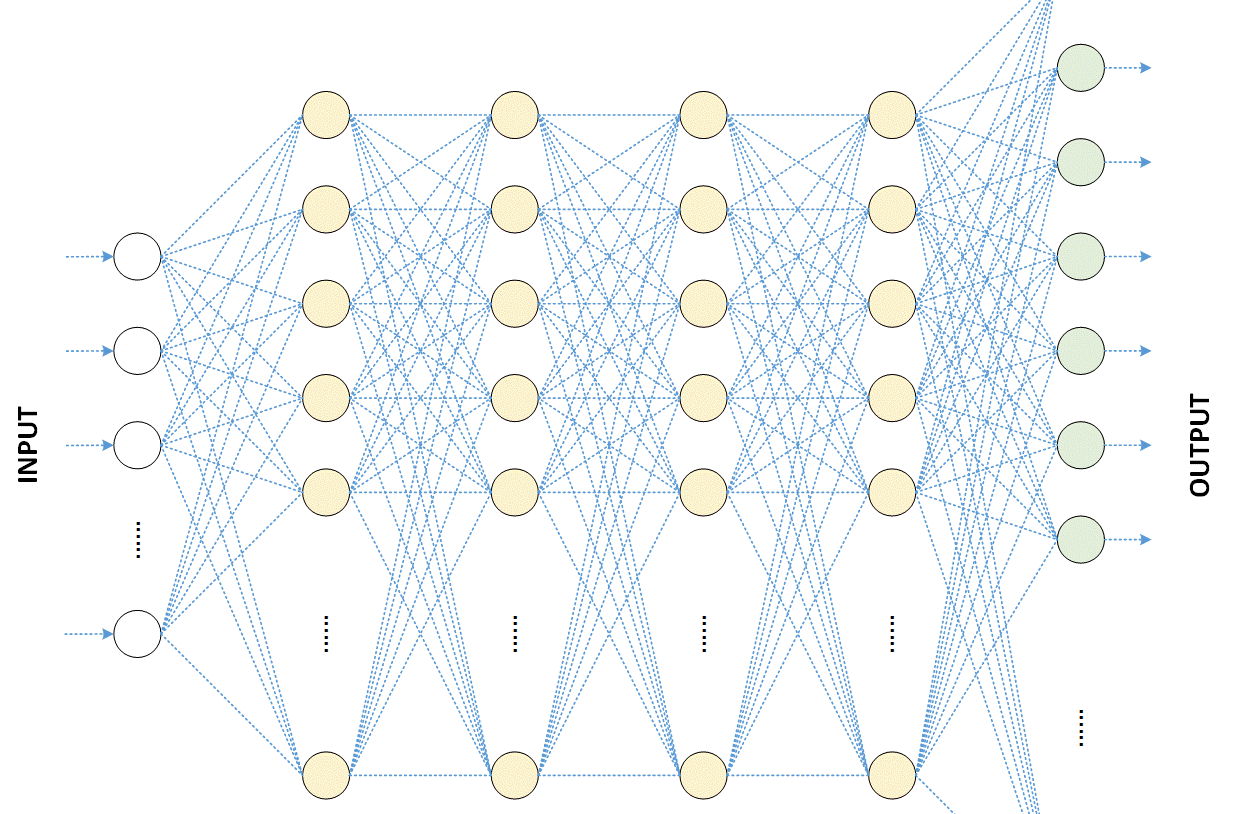
\includegraphics[width=0.65\linewidth]{network_dnn}
	\caption[]{\label{fig:network_dnn}
	DNN网络模型
	}
\end{figure}

\paragraph{深度学习框架}\cite{ wiki:Deep_learning}至今已有数种深度学习框架。包括深度神经网络、卷积神经网络和深度置信网络和递归神经网络。深度学习在计算机视觉、自然语言处理等方面已经取得了极好的效果。本文涉及的问题属于计算机视觉领域,深度学习的优越性正是选择的初衷。

深度神经网络是一种具备至少一个隐层的神经网络。深度神经网络具有更多网络层,如\cref{fig:network_dnn}示例,一般来说第一层是输入层,中间的层数为隐藏层,最后一层是输出层。

\paragraph{递归神经网络}\cite{ wiki:RNN}(Recurrent Neural Network,RNN)是一种节点定向连接成环的人工神经网络,属于深度学习网络的一种。
\begin{itemize}
  \item \textbf{编码器}递归神经网络将输入序列$\vec{x}$编码为一个固定长度的隐藏状态$\vec{h}$(以自然语言处理为例)
  \begin{itemize}
    \item $\vec{x}=\left(x_{t}, \ldots, x_{1}\right)$是输入序列。
    \item $\overrightarrow{h_{t}}=f\left(x_{t}, \overrightarrow{h_{t-1}}\right)$ 是随时间更新的隐藏状态。之前的状态$\overrightarrow{h_{t-1}}$转换为和当前输入$x_t$相关的$\overrightarrow{h_{t}}$。
  \end{itemize}
  其中,计算隐藏状态的方程$f(x,h)$是一个非线性方程,可以是复杂的\textbf{LSTM}单元(Long-ShortTerm Memory)。获得隐藏状态序列后,做出下一步预测:
  \begin{itemize}
    \item $p\left(y_{t}\right)=p\left(y_{t} | y_{t-1}, \ldots, y_{1}\right)$,其中$y_{t}$是第$t$个位置上的输出。
    \item 以上概率可以通过隐藏状态来计算:$p\left(y_{t}\right)=g\left(y_{t-1}, \overrightarrow{h_{t}}, \vec{c}\right), \vec{c}$是所有隐藏状态的编码,总含了所有隐藏状态。因为隐藏状态$t$就编码了第$t$个输入前全部的输入信息,$y_{t}$也迭代式地隐含了之前的全部输出信息。
  \end{itemize}
  \item \textbf{解码器}神经网络可以添加编码器作为解码器($Decoder$)。编码后($Encoded$)的信息通过解码器翻译为人类熟悉的信息。也就是上述例子中的$y_{t}=f\left(y_{t-1}, h_{t}, c\right)$过程,当中非线性模型$f$就是作为输出的复发神经网络。同时需要对$h_t^{'}$继续进行迭代:
  \begin{itemize}
    \item $h_{t}^{\prime}=g\left(h_{t-1}, y_{t-1}, c\right), \vec{c}$是解码器传递给编码器的参数,是解码器中状态的summary。$h_t^{'}$是解码器的隐藏状态。$y_t$是第$t$个输出。
    \item 当输入仍为$\vec{x}=\left(x_{t}, \ldots, x_{1}\right)$,输出是$\vec{y}=\left(y_{t}, \ldots, y_{1}\right)$,最大化条件概率$P(\vec{y} | \vec{x})$就是最好的结果。
  \end{itemize}
\end{itemize}

% \begin{figure}
% \centering
% \subfigure[RNN(左侧)和LSTM(右侧)对比] {
% \label{fig:lstm_rnn}
% 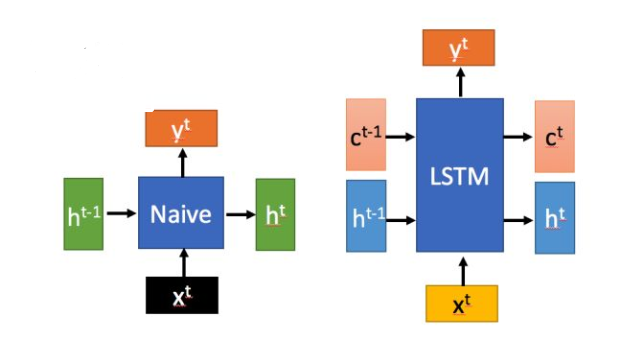
\includegraphics[width=0.65\textwidth]{lstm_rnn}
% }
% \subfigure[LSTM状态] {
% \label{fig:lstm_state}
% 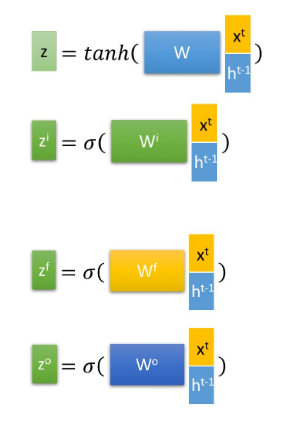
\includegraphics[width=0.3\textwidth]{lstm_fourstate}
% }
% \subfigure[LSTM内部结构] {
% \label{fig:lstm_inside}
% 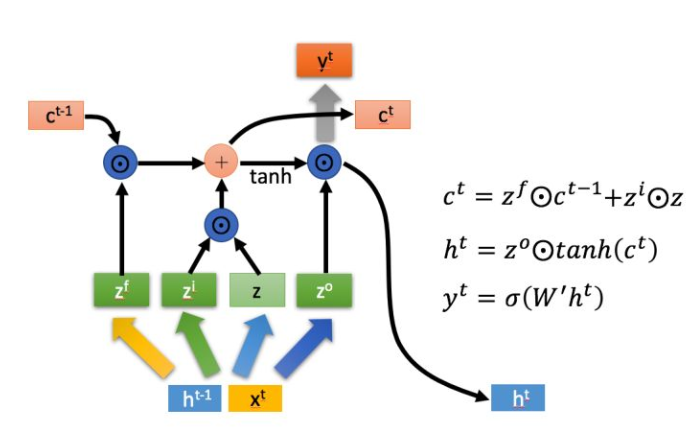
\includegraphics[width=\textwidth]{lstm_inside}
% }
% \end{figure}

\paragraph{长短期记忆}\cite{ wiki:LSTM}($Long short-term memory$, LSTM)是人工递归神经网络(RNN)的一种模式,广泛地运用于深度学习领域。与标准的前馈神经网络不同,LSTM具有反馈机制。LSTM不仅可以处理单个数据点,也可以处理整个数据序列。

一个通用的LSTM单元由单元,输入门,输出门和遗忘门组成。单元负责记住任意时间间隔内的值。三个门控制进出单元的信息流。

LSTM非常适合于对时间序列数据的分类任务、处理任务等。因为在时间序列中,重要事件之间可能存在未知的滞后和联系。LSTM提出的初衷就是为了处理在训练传统RNN时可能遇到的梯度爆炸和梯度消失问题。LSTM的优势还在于该网络对于间隙长度的不敏感性。

\begin{itemize}
  \item LSTM架构有很多种。常见的LSTM架构由单元(LSTM单元的存储器部分)和LSTM单元内部信息流的三个“调节器”组成:输入门,输出门和遗忘门。 一些变形的LSTM单元可能不具有一个或多个门,或者可能具有其他类型的门。单元负责跟踪输入序列中的元素之间的依赖性。输入门控制新值流入单元的程度,忘记门控制值在单元中保留的程度,输出门中的值用于计算输出的程度从而激活LSTM单元。 LSTM门的激活功能通常是逻辑功能。
  \item 具有遗忘门的LSTM单元的正向通过的形式如下:
  \begin{equation}
    \begin{aligned} f_{t} &=\sigma_{g}\left(W_{f} x_{t}+U_{f} h_{t-1}+b_{f}\right) \\ i_{t} &=\sigma_{g}\left(W_{i} x_{t}+U_{i} h_{t-1}+b_{i}\right) \\ o_{t} &=\sigma_{g}\left(W_{o} x_{t}+U_{o} h_{t-1}+b_{o}\right) \\ c_{t} &=f_{t} \circ c_{t-1}+i_{t} \circ \sigma_{c}\left(W_{c} x_{t}+U_{c} h_{t-1}+b_{c}\right) \\ h_{t} &=o_{t} \circ \sigma_{h}\left(c_{t}\right) \end{aligned}
  \end{equation}其中初始值为$c_ {0} = 0$且$h_ {0} = 0$和运算符$\circ$表示$Hadamard$。下标$t$为时间步长。
  式子中变量定义如下:
  \begin{itemize}
    \item $x_{t} \in \mathbb{R}^{d}$:LSTM单元的输入向量。
    \item $f_{t} \in \mathbb{R}^{h}$:遗忘门的激活向量。
    \item $i_{t} \in \mathbb{R}^{h}$:输入门的激活向量。
    \item $o_{t} \in \mathbb{R}^{h}$:输出门的激活向量。
    \item $h_{t} \in \mathbb{R}^{h}$:隐藏状态向量,也称为LSTM单元的输出向量。
    \item $c_{t} \in \mathbb{R}^{h}$:单元状态向量。
    \item $W \in \mathbb{R}^{h \times d}, U \in \mathbb{R}^{h \times h}$ 和 $b \in \mathbb{R}^{h}$:权重矩阵和偏差参数。
  \end{itemize}
  式子中的激活函数如下:
  \begin{itemize}
    \item $\sigma_{g}$:$sigmoid$ 函数。
    \item $\sigma_{c}$:双曲正切函数。
    \item $\sigma_{h}$:双曲正切函数。
  \end{itemize}
\end{itemize}
